\documentclass[12pt,hyperref=true,mathserif]{beamer}

% Package and Theme
\usepackage{amsmath}
% I suppose listings is no longer needed.
% \usepackage{listings}
\usetheme{AnnArbor}
\graphicspath{{Figure/}{figures/}{figure/}{pictures/}{picture/}{pic/}{pics/}}

% Document Begin
\begin{document}
\title{Revenge of the Nerds}
\author{Yanan Xiao}
\institute[Masdar Institute]{Masdar Institute of Science and
  Technology}
\date[CIS502 Presentation]{Software Engineering Course Presentation}

% Frame Begin
\begin{frame}
\titlepage
\end{frame}

\begin{frame}
  \tableofcontents
\end{frame}

\section{Introduction}


\begin{frame}
% \centering
\begin{center}
``Programming languages have almost caught up with 1958.''
\end{center}
\hfill  Paul Graham  
\end{frame}

\begin{frame}
  \frametitle{A Bit of History}
  \begin{columns}
    \begin{column}{0.5\textwidth}
      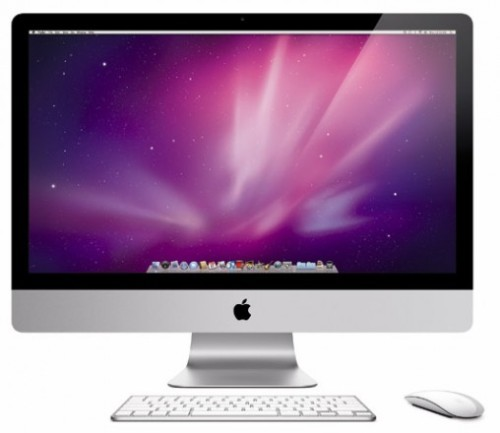
\includegraphics[scale=0.3]{iMac-500}
    \end{column}
    \begin{column}{0.5\textwidth}
      Question about \emph{computation}.\\[4pt]
      If we had machines that have infinite computational power, what
      problems would we be able to solve?
    \end{column}
  \end{columns}
  
\end{frame}

\begin{frame}
  Lambda calculus.
  \begin{itemize}
  \item A formal system developed by Alonzo Church.
  \item Essentially a programming language for one of those imaginary
    machines.
  \item Equivalent in power with Turing Machine.
  \end{itemize}
  Lisp.
  \begin{itemize}
  \item Invented by John McCarthy as an implementation of Alonzo's
    lambda calculus, in 1958.
  \item Lisp machine developed by programmers from MIT AI lab, as a
    native hardware implementation.
  \end{itemize}
\end{frame}

\section{Functional Programming at a Glimpse}


\begin{frame}
  
\end{frame}

\section{More Details}


\begin{frame}
  
\end{frame}

\section{Dream Language}


\begin{frame}
  
\end{frame}





\end{document}


% Someone like you.
